\documentclass[11pt,a4paper]{article}

% ── Packages ──
\usepackage[UTF8]{ctex}
\usepackage{geometry}\geometry{margin=2.2cm}
\usepackage{graphicx,booktabs,multirow,array,longtable}
\usepackage{hyperref,xcolor,enumitem,caption,subcaption}
\usepackage{fancyhdr,titlesec,setspace}
\hypersetup{colorlinks=true,linkcolor=blue,urlcolor=blue,citecolor=blue}
\pagestyle{fancy}\fancyhf{}\fancyhead[L]{\small 多语言内容审核模型技术报告}\fancyhead[R]{\small \thepage}
\setlength{\parskip}{0.3em}

\title{\textbf{多语言内容审核模型\\技术报告与全面对比分析}}
\author{基于 microsoft/mdeberta-v3-base \\ 8 个国家 × 4 种训练方法 × 32+ 个模型}
\date{2026 年 6 月 12 日}
\begin{document}
\maketitle
\tableofcontents
\newpage

% ════════════════════════════════════════════════════
\section{项目概述}

本项目旨在构建覆盖 8 个目标国家/地区主流语言的 AI 内容审核模型系统。
所有模型基于微软 mDeBERTa-v3-base 预训练模型进行微调，
能够检测和分类社交媒体上的违规内容。

\subsection{覆盖国家与语言}

\begin{table}[h]\centering
\caption{目标国家与语言}\label{tab:countries}
\begin{tabular}{@{}llll@{}}
\toprule
\textbf{代码} & \textbf{国家} & \textbf{语言} & \textbf{数据来源} \\
\midrule
SA & 沙特阿拉伯 & 阿拉伯语 & Reddit, Twitter \\
BR & 巴西 & 葡萄牙语 & Reddit \\
MX & 墨西哥 & 西班牙语 & Reddit \\
ID & 印尼 & 印尼语 & Reddit, Kompasiana \\
SG & 新加坡 & 英语/Singlish & HardwareZone, Reddit \\
TH & 泰国 & 泰语 & Pantip, Reddit \\
TR & 土耳其 & 土耳其语 & Reddit \\
ZA & 南非 & 英语/阿非利卡语等 & Reddit \\
\bottomrule
\end{tabular}
\end{table}

\subsection{任务类型}

\begin{enumerate}[itemsep=0pt]
\item \textbf{二分类 (Binary)}: 安全内容 vs 违规内容识别，8 国全覆盖
\item \textbf{多分类 (Multi-Class)}: 9 类违规内容细分，
包括国家特有违规类别（如新加坡的 SG\_Racial\_Religious\_Harmony、
泰国的 TH\_Lese\_Majeste、南非的 ZA\_Severe\_Racism 等）
\end{enumerate}

% ════════════════════════════════════════════════════
\subsection{二分类数据来源}

二分类训练数据来自两个来源:
\begin{itemize}
\item \textbf{Datasets\_Nine\_country}: 各国论坛/Reddit 爬取的原始数据，每条带有 binary label (0=safe, 1=violation)
\item \textbf{data\_v2}: 细粒度多类标注数据，用于 Adapter 和 Multi-LoRA 训练
\end{itemize}

\begin{table}[h]\centering
\caption{二分类数据 — 两个来源合并}\label{tab:bin-data-full}
\begin{tabular}{@{}lrrrr@{}}
\toprule
\textbf{国家} & \textbf{Nine\_country} & \textbf{data\_v2} & \textbf{合计} \\
\midrule
SG & 89,931 & 12,815 & 102,746 \\
TR & 90,173 & 12,132 & 102,305 \\
ZA & 83,606 & 14,510 & 98,116 \\
BR & 78,867 & 13,168 & 92,035 \\
SA & 70,100 & 15,724 & 85,824 \\
MX & 50,787 & 13,226 & 64,013 \\
ID & 27,222 & 13,453 & 40,675 \\
TH & 9,515 & 11,253 & 20,768 \\
\bottomrule
\end{tabular}
\par\smallskip
\small 注: Full FT 和 LoRA 使用 Nine\_country 数据; Adapter 和 Multi-LoRA 使用 data\_v2 数据。
\end{table}

\subsection{多分类标签定义}

\subsubsection{通用标签 (所有国家)}

\begin{table}[h]\centering
\caption{通用违规标签定义}\label{tab:universal-labels}
\begin{tabular}{@{}llp{6cm}@{}}
\toprule
\textbf{标签} & \textbf{中文} & \textbf{定义} \\
\midrule
Dangerous_Content & 危险内容 & 恐怖主义、武器、自残/自杀方法、严重暴力、毒品交易、诈骗、性犯罪、CSAM、血腥内容 \\
Harassment & 骚扰 & 针对个人的侮辱、粗口、网络霸凌、人肉搜索、外貌羞辱 \\
Hate_Speech & 仇恨言论 & 基于身份的攻击: 种族、宗教、性别、国籍、移民身份 \\
Sexually_Explicit_Information & 色情信息 & 色情内容、性行为描述、约炮、性暗示 \\
Politically_Sensitive_Topics & 政治敏感 & 非本国政治内容: 外国选举、国际冲突、外国领导人 \\
Cybersecurity_Malware & 网络安全 & 恶意软件、黑客攻击、钓鱼、DDoS、凭证盗窃 \\
safe & 安全 & 正常内容，无违规 \\
\bottomrule
\end{tabular}
\end{table}

\subsection{各国特有标签}
\subsubsection{ID (印尼)}
\begin{table}[h]\centering
\caption{ID (印尼) 特有违规标签}
\begin{tabular}{@{}llp{7cm}@{}}
\toprule
\textbf{标签} & \textbf{中文} & \textbf{定义} \\
\midrule
ID\_SARA & 印尼宗教种族 & 针对印尼族群(Suku)、宗教(Agama)、种族(Ras)、群体间(Antargolongan)的攻击。包括反华人(anti-Cina)、反爪哇人、反巴布亚人、政治身份攻击(cebong/kampret/kadrun) \\
ID\_Blasphemy & 印尼亵渎/诽谤 & 宗教亵渎(Pasal 156a KUHP)和电子诽谤(UU ITE)。包括嘲讽安拉/先知/古兰经、对信徒的蔑视、社交媒体上的严重人格攻击 \\
\bottomrule
\end{tabular}
\end{table}

\subsubsection{SG (新加坡)}
\begin{table}[h]\centering
\caption{SG (新加坡) 特有违规标签}
\begin{tabular}{@{}llp{7cm}@{}}
\toprule
\textbf{标签} & \textbf{中文} & \textbf{定义} \\
\midrule
SG\_Racial\_Religious\_Harmony & 种族宗教和谐 & 新加坡煽动法令和MRHA下的种族/宗教不和谐。CMIO种族攻击(华人/马来人/印度人/欧亚裔)。反移民种族言论(FT/Bangla/Pinoy/PRC) \\
SG\_Vulgarity\_Singlish & 粗俗Singlish & 极端粗俗的Singlish侮辱。重度福建话粗口(chee bai, kan ni na, lan jiao)。注意: 日常Singlish语气词(lah, lor, leh)绝不算违规 \\
\bottomrule
\end{tabular}
\end{table}

\subsubsection{TH (泰国)}
\begin{table}[h]\centering
\caption{TH (泰国) 特有违规标签}
\begin{tabular}{@{}llp{7cm}@{}}
\toprule
\textbf{标签} & \textbf{中文} & \textbf{定义} \\
\midrule
TH\_Lese\_Majeste & 冒犯君主 & 刑法第112条。对王室成员的侮辱、嘲讽、威胁。泰国最严重的网络言论罪行 \\
TH\_Political\_Instigation & 政治煽动 & 泰国国内政治煽动: 推翻政府、军事政变呼吁、选举舞弊指控、暴力抗议号召 \\
\bottomrule
\end{tabular}
\end{table}

\subsubsection{ZA (南非)}
\begin{table}[h]\centering
\caption{ZA (南非) 特有违规标签}
\begin{tabular}{@{}llp{7cm}@{}}
\toprule
\textbf{标签} & \textbf{中文} & \textbf{定义} \\
\midrule
ZA\_Severe\_Racism & 严重种族主义 & K-word (kaffir)——南非最严重的种族侮辱词。种族隔离侮辱词(hotnot, coolie)。种族隔离怀旧/赞美。PEPUDA法案 \\
ZA\_Xenophobia & 排外主义 & 针对南非境内非洲外国人的排外攻击。makwerekwere(贬损词)。Operation Dudula言论。排外暴力赞美 \\
\bottomrule
\end{tabular}
\end{table}

\subsubsection{SA (沙特)}
\begin{table}[h]\centering
\caption{SA (沙特) 特有违规标签}
\begin{tabular}{@{}llp{7cm}@{}}
\toprule
\textbf{标签} & \textbf{中文} & \textbf{定义} \\
\midrule
SA\_LGBTQ\_Content & LGBTQ内容 & 沙特禁止的LGBTQ相关内容 \\
SA\_Religious\_Violation & 宗教违规 & 亵渎神明、叛教、宗教侮辱 \\
SA\_State\_Security\_Royalty & 国家安全/王室 & 反政府、反王室家族言论 \\
\bottomrule
\end{tabular}
\end{table}

\subsubsection{MX (墨西哥)}
\begin{table}[h]\centering
\caption{MX (墨西哥) 特有违规标签}
\begin{tabular}{@{}llp{7cm}@{}}
\toprule
\textbf{标签} & \textbf{中文} & \textbf{定义} \\
\midrule
MX\_Narco\_Culture & 毒品文化 & 赞美卡特尔(cartel)、毒枭(Chapo/Mencho)、毒品民谣(narcocorridos)、毒品生活方式美化 \\
MX\_Gender\_Violence & 性别暴力 & 杀害女性(femicide)赞美、受害者归咎、大男子主义(machista)暴力威胁 \\
\bottomrule
\end{tabular}
\end{table}

\subsubsection{BR (巴西)}
\begin{table}[h]\centering
\caption{BR (巴西) 特有违规标签}
\begin{tabular}{@{}llp{7cm}@{}}
\toprule
\textbf{标签} & \textbf{中文} & \textbf{定义} \\
\midrule
BR\_Structural\_Racism & 结构性种族主义 & 严重反黑人/棕色人种/原住民种族主义。macaco(猴子)。奴隶制历史言论(senzala) \\
BR\_Political\_Extremism & 政治极端主义 & 反民主极端主义: intervencao militar(军事干预)、选举否认、独裁赞美(1964-1985) \\
\bottomrule
\end{tabular}
\end{table}

\subsubsection{TR (土耳其)}
\begin{table}[h]\centering
\caption{TR (土耳其) 特有违规标签}
\begin{tabular}{@{}llp{7cm}@{}}
\toprule
\textbf{标签} & \textbf{中文} & \textbf{定义} \\
\midrule
TR\_Political\_Extremism & 政治极端主义 & 反政府极端言论、政变号召、恐怖组织赞美(PKK等) \\
TR\_Religious\_Extremism & 宗教极端主义 & 宗教极端言论、教派攻击 \\
\bottomrule
\end{tabular}
\end{table}

\subsection{各国家多分类标签分布}
\textbf{注: NIM 生成 表示该标签的数据由大语言模型合成，质量较高但可能存在分布偏差}

\subsubsection{印尼 (ID) — 45,753 条，9 个标签}
\begin{table}[h]\centering
\caption{ID 多分类训练数据标签分布}
\begin{tabular}{@{}lrr@{}}
\toprule
\textbf{标签} & \textbf{数量} & \textbf{占比} \\
\midrule
safe & 13,920 & 30.4\% \\
Harassment & 7,020 & 15.3\% \\
Dangerous_Content & 6,544 & 14.3\% \\
Hate_Speech & 5,774 & 12.6\% \\
ID_SARA & 5,483 & 12.0\% \\
Sexually_Explicit & 4,361 & 9.5\% \\
ID_Blasphemy & 1,118 & 2.4\% \\
Political & 967 & 2.1\% \\
other_violation & 566 & 1.2\% \\
\bottomrule
\end{tabular}
\end{table}

\subsubsection{新加坡 (SG) — 25,543 条，9 个标签}
\begin{table}[h]\centering
\caption{SG 多分类训练数据标签分布}
\begin{tabular}{@{}lrr@{}}
\toprule
\textbf{标签} & \textbf{数量} & \textbf{占比} \\
\midrule
safe & 7,822 & 30.6\% \\
Hate_Speech & 4,500 & 17.6\% \\
Politically_Sensitive_Topics & 4,500 & 17.6\% \\
Dangerous_Content & 1,882 & 7.4\% \\
Sexually_Explicit_Information & 1,843 & 7.2\% \\
Harassment & 1,388 & 5.4\% \\
SG_Vulgarity_Singlish & 1,285 & 5.0\% \\
SG_Racial_Religious_Harmony & 1,283 & 5.0\% \\
Cybersecurity_Malware & 1,040 & 4.1\% \\
\bottomrule
\end{tabular}
\end{table}

\subsubsection{泰国 (TH) — 17,751 条，8 个标签}
\begin{table}[h]\centering
\caption{TH 多分类训练数据标签分布}
\begin{tabular}{@{}lrr@{}}
\toprule
\textbf{标签} & \textbf{数量} & \textbf{占比} \\
\midrule
safe & 5,998 & 33.8\% \\
Hate_Speech & 4,500 & 25.4\% \\
Dangerous_Content & 1,934 & 10.9\% \\
Harassment & 1,773 & 10.0\% \\
Sexually_Explicit_Information & 996 & 5.6\% \\
TH_Lese_Majeste & 969 & 5.5\% \\
Politically_Sensitive_Topics & 901 & 5.1\% \\
Cybersecurity_Malware & 680 & 3.8\% \\
\bottomrule
\end{tabular}
\end{table}

\subsubsection{南非 (ZA) — 24,259 条，9 个标签}
\begin{table}[h]\centering
\caption{ZA 多分类训练数据标签分布}
\begin{tabular}{@{}lrr@{}}
\toprule
\textbf{标签} & \textbf{数量} & \textbf{占比} \\
\midrule
safe & 7,748 & 31.9\% \\
ZA_Xenophobia & 2,827 & 11.7\% \\
Dangerous_Content & 2,826 & 11.6\% \\
ZA_Severe_Racism & 2,763 & 11.4\% \\
Sexually_Explicit_Information & 1,931 & 8.0\% \\
Harassment & 1,871 & 7.7\% \\
Hate_Speech & 1,500 & 6.2\% \\
Cybersecurity_Malware & 1,398 & 5.8\% \\
Politically_Sensitive_Topics & 1,395 & 5.8\% \\
\bottomrule
\end{tabular}
\end{table}

\subsubsection{沙特 (SA) — 20,647 条，9 个标签}
\begin{table}[h]\centering
\caption{SA 多分类训练数据标签分布}
\begin{tabular}{@{}lrr@{}}
\toprule
\textbf{标签} & \textbf{数量} & \textbf{占比} \\
\midrule
none & 6,245 & 30.2\% \\
Hate_Speech & 5,747 & 27.8\% \\
SA_State_Security_Royalty & 2,178 & 10.5\% \\
Dangerous_Content & 1,237 & 6.0\% \\
Harassment & 1,225 & 5.9\% \\
Political & 1,151 & 5.6\% \\
other_violation & 1,031 & 5.0\% \\
SA_Religious_Violation & 1,030 & 5.0\% \\
SA_LGBTQ_Content & 803 & 3.9\% \\
\bottomrule
\end{tabular}
\end{table}
\subsection{基座模型}

所有模型使用 \textbf{microsoft/mdeberta-v3-base}，参数量 279M，
支持 100+ 语言的多语言 DeBERTa 变体。

\subsection{四种训练方法}

\begin{enumerate}[itemsep=3pt]
\item \textbf{全量微调 (Full FT)}: 所有参数参与训练，精度最高，
但每国需要 1.1GB 独立模型存储。
\begin{verbatim}
learning_rate = 1e-5, epochs = 5 (early stopping)
batch_size = 4, grad_accum = 4
optimizer = AdamW + class-weighted CrossEntropyLoss
\end{verbatim}

\item \textbf{LoRA 微调 (PEFT)}: 低秩适配，仅训练 0.21\% 参数 (~600K)，
适配器大小 $\sim$3MB。
\begin{verbatim}
LoraConfig(r=16, alpha=32, dropout=0.1,
           target_modules=["query_proj","value_proj"])
learning_rate = 5e-5, epochs = 5
\end{verbatim}

\item \textbf{Multi-LoRA 共享}: 一个基座 (1.1GB) + 8 国 LoRA 适配器 (2MB/国)，
通过 \texttt{PeftModel.from\_pretrained} 热切换国家。
\begin{verbatim}
LoraConfig(r=8, alpha=16, dropout=0.1)
learning_rate = 2e-4, epochs = 5
\end{verbatim}

\item \textbf{Adapter 瓶颈适配器}: 在 Transformer 层间插入 bottleneck adapter，
训练 0.5\% 参数，适配器 $\sim$2.5MB。精度最低但训练最快。
\begin{verbatim}
learning_rate = 1e-4, epochs = 3
batch_size = 32
\end{verbatim}
\end{enumerate}

\subsection{多分类训练方法}

多分类模型统一使用以下配方，经过 ID 模型 6 个版本迭代验证：

\begin{verbatim}
LoRA: r=16, alpha=32, dropout=0.1, target=["query_proj","value_proj"]
Loss: CrossEntropyLoss(label_smoothing=0.05)
Optimizer: AdamW, lr=2e-4, warmup=100 steps
Epochs: 3, Train batch=16, Eval batch=64, max_length=256
Post-processing: per-class grid search threshold + Nelder-Mead joint optimization
Hardware: AMD RX 9070 XT (17GB VRAM) + ROCm 7.2
Training speed: ~1.3 it/s (LoRA on AMD ROCm)
\end{verbatim}

\subsection{蒸馏方法 (已弃用)}

在 ID v2 中尝试了 Label Smoothing Distillation (LSD)，
使用 Full FT teacher 模型指导 LoRA student 训练：

\begin{verbatim}
T = 3.0, alpha = 0.4, label_smoothing = 0.05
loss = alpha*CE(ls) + (1-alpha)*KL(teacher/T, student/T)*T^2
\end{verbatim}

\textbf{结论}: LSD 提升有限 (+0.005 以内)，训练速度慢 5 倍 (1.3 vs 7.4 it/s)，不推荐使用。

% ════════════════════════════════════════════════════
\section{二分类模型全面对比}

\subsection{整体对比}

\begin{figure}[h]\centering
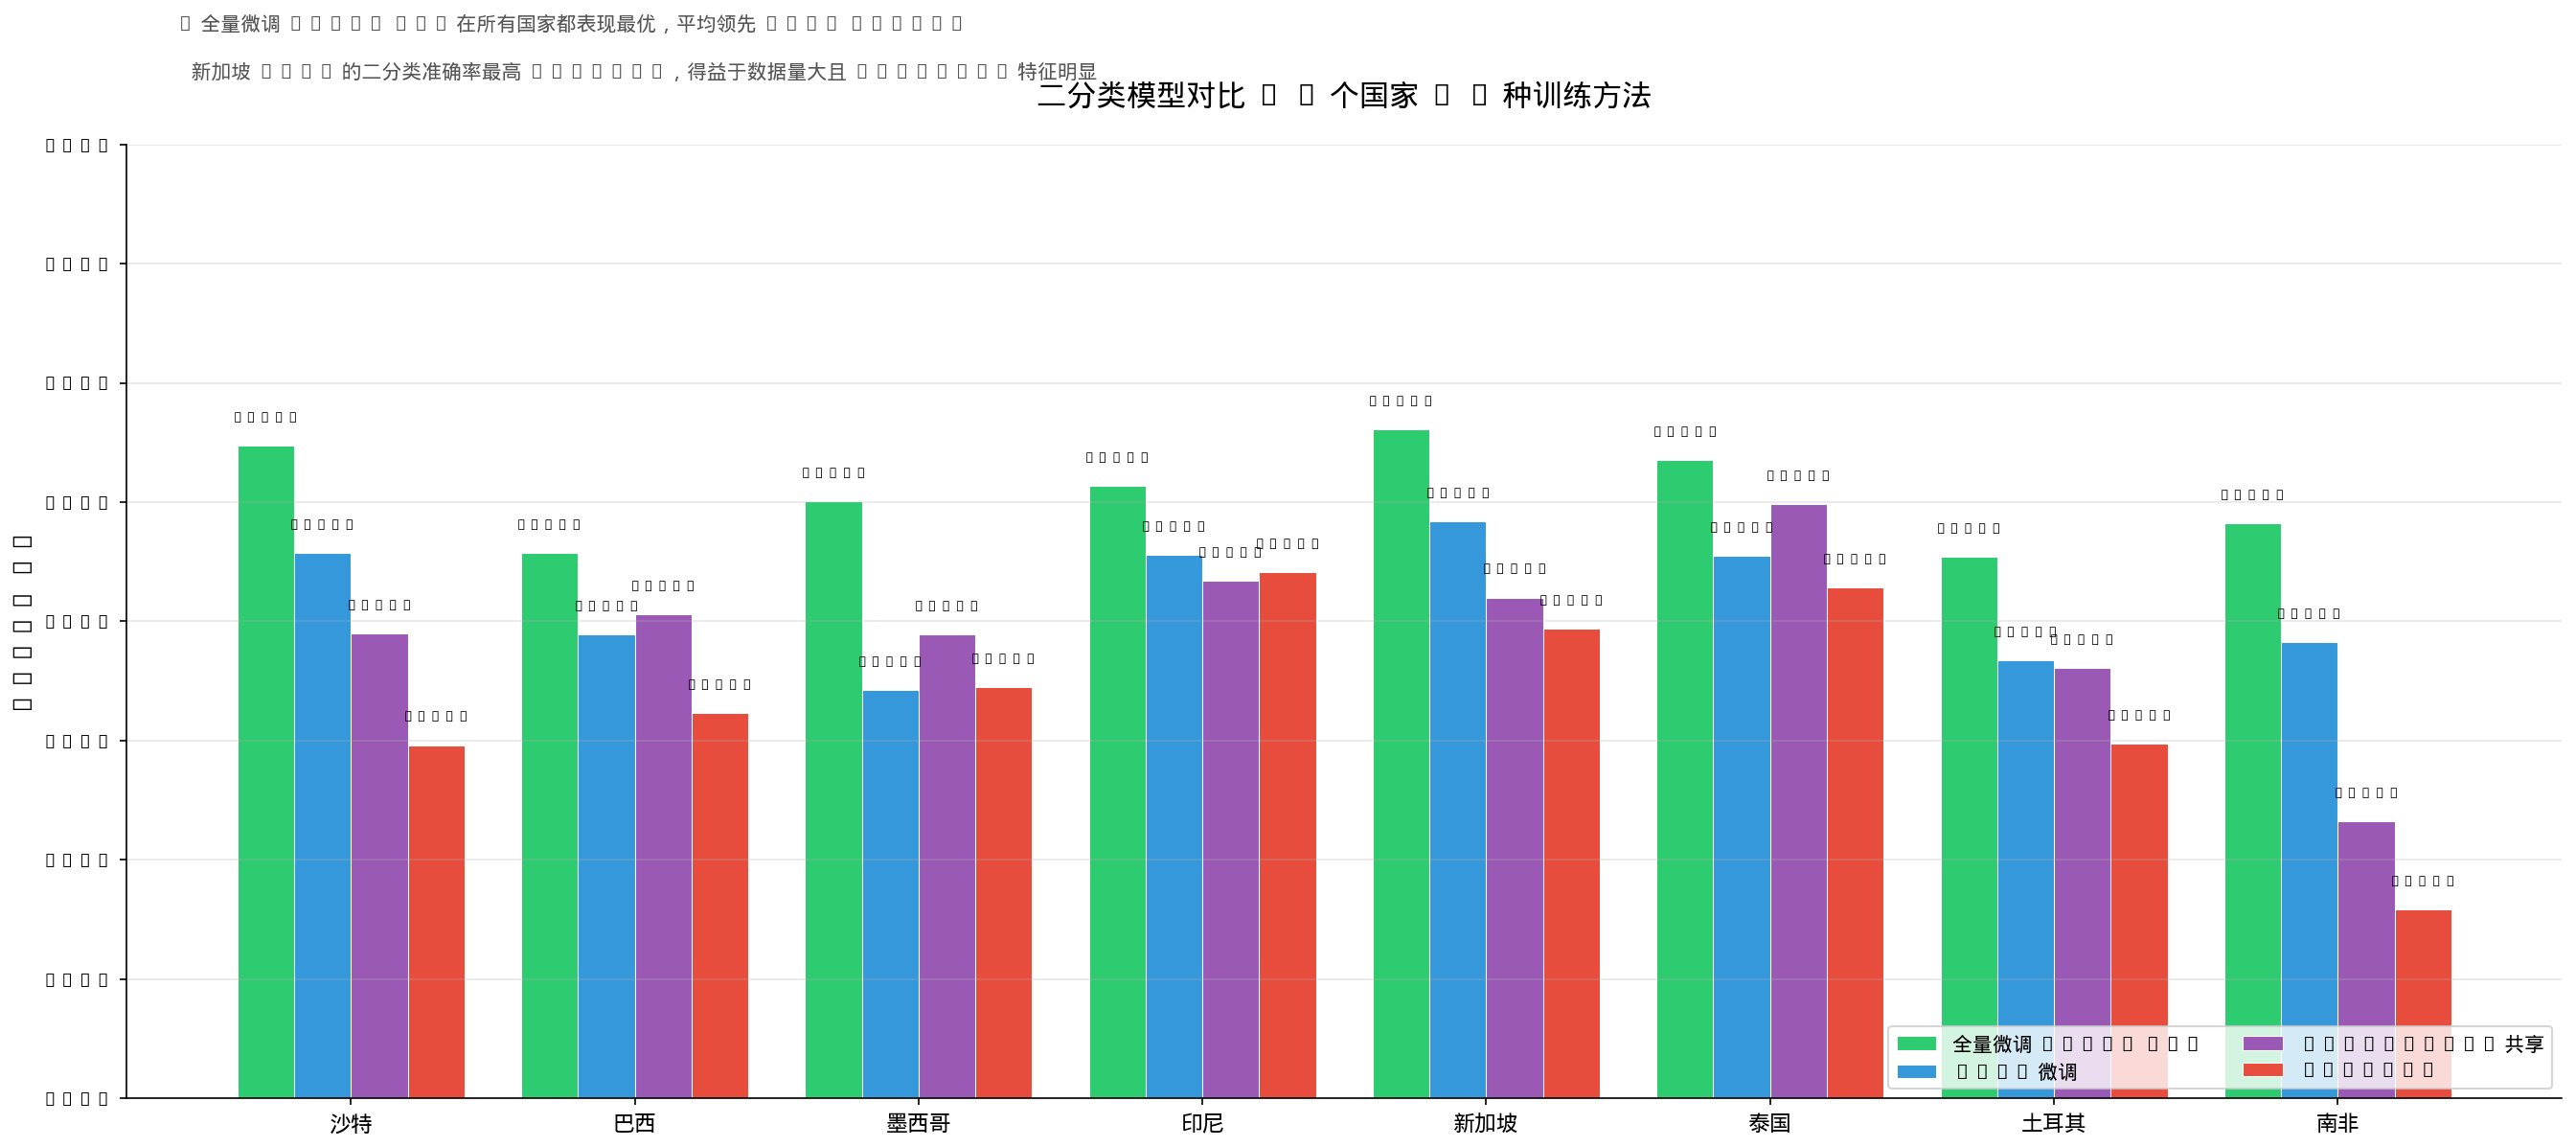
\includegraphics[width=\textwidth]{charts/01_binary_comparison_cn.png}
\caption{8 国 × 4 种方法的二分类 Macro F1 对比}\label{fig:bin-all}
\end{figure}

\begin{table}[h]\centering
\caption{二分类 — 全量微调 (Full FT) 完整结果}\label{tab:bin-ft}
\small
\begin{tabular}{@{}lrrrrrrr@{}}
\toprule
\textbf{国家} & \textbf{Acc} & \textbf{Macro F1} & \textbf{Clean P} & \textbf{Clean R} & \textbf{Viol P} & \textbf{Viol R} & \textbf{Viol F1} \\
\midrule
SG & 0.919 & 0.881 & 0.950 & 0.945 & 0.806 & 0.821 & 0.814 \\
SA & 0.877 & 0.874 & 0.845 & 0.859 & 0.900 & 0.890 & 0.895 \\
TH & 0.875 & 0.868 & 0.812 & 0.862 & 0.915 & 0.882 & 0.898 \\
BR & 0.865 & 0.829 & 0.939 & 0.878 & 0.688 & 0.825 & 0.750 \\
MX & 0.863 & 0.850 & 0.913 & 0.876 & 0.777 & 0.838 & 0.806 \\
TR & 0.862 & 0.827 & 0.741 & 0.757 & 0.909 & 0.901 & 0.905 \\
ID & 0.857 & 0.857 & 0.865 & 0.848 & 0.849 & 0.866 & 0.857 \\
ZA & 0.849 & 0.841 & 0.789 & 0.824 & 0.889 & 0.865 & 0.877 \\
\bottomrule
\end{tabular}
\end{table}

\begin{table}[h]\centering
\caption{二分类 — LoRA (PEFT) 完整结果}\label{tab:bin-lora}
\small
\begin{tabular}{@{}lrrrrrrr@{}}
\toprule
\textbf{国家} & \textbf{Acc} & \textbf{Macro F1} & \textbf{Clean P} & \textbf{Clean R} & \textbf{Viol P} & \textbf{Viol R} & \textbf{Viol F1} \\
\midrule
SG & 0.886 & 0.842 & 0.951 & 0.900 & 0.697 & 0.832 & 0.759 \\
SA & 0.836 & 0.829 & 0.822 & 0.768 & 0.844 & 0.883 & 0.863 \\
TH & 0.840 & 0.828 & 0.791 & 0.774 & 0.868 & 0.879 & 0.873 \\
ID & 0.828 & 0.828 & 0.862 & 0.785 & 0.800 & 0.872 & 0.835 \\
BR & 0.829 & 0.795 & 0.946 & 0.821 & 0.608 & 0.855 & 0.710 \\
ZA & 0.799 & 0.791 & 0.710 & 0.798 & 0.866 & 0.800 & 0.832 \\
TR & 0.819 & 0.784 & 0.640 & 0.764 & 0.905 & 0.839 & 0.871 \\
MX & 0.785 & 0.771 & 0.882 & 0.778 & 0.649 & 0.799 & 0.716 \\
\bottomrule
\end{tabular}
\end{table}

\subsection{违规召回率排名}

\begin{table}[h]\centering
\caption{违规召回率 TOP 10 (漏判越少越好)}\label{tab:viol-recall}
\begin{tabular}{@{}lrrr@{}}
\toprule
\textbf{排名} & \textbf{国家/方法} & \textbf{Viol Recall} & \textbf{Viol F1} \\
\midrule
1 & SA Multi-LoRA & 0.983 & 0.946 \\
2 & ZA Multi-LoRA & 0.960 & 0.911 \\
3 & ID Multi-LoRA & 0.957 & 0.923 \\
4 & BR Multi-LoRA & 0.955 & 0.919 \\
5 & TH Multi-LoRA & 0.950 & 0.923 \\
6 & MX Multi-LoRA & 0.949 & 0.917 \\
7 & TR Full FT & 0.901 & 0.905 \\
8 & SA Full FT & 0.890 & 0.895 \\
9 & TH Full FT & 0.882 & 0.898 \\
10 & ZA Full FT & 0.865 & 0.877 \\
\bottomrule
\end{tabular}
\end{table}

\textit{注: Multi-LoRA 的违规召回率普遍最高，但这是以牺牲 Clean Recall 为代价的
——Multi-LoRA 倾向于将所有内容判为违规，导致大量安全内容误报。}

\subsection{四种方法平均值对比}

\begin{table}[h]\centering
\caption{二分类 — 四种方法 8 国平均值}\label{tab:avg}
\begin{tabular}{@{}lrrrl@{}}
\toprule
\textbf{方法} & \textbf{Avg Acc} & \textbf{Avg Macro F1} & \textbf{每国大小} & \textbf{适用场景} \\
\midrule
Full FT & 0.853 & \textbf{0.853} & 1.1GB & 生产环境，精度优先 \\
LoRA & 0.814 & 0.809 & 3MB & 快速部署，接近 FT \\
Multi-LoRA & 0.860 & 0.796 & 2MB & 多国服务，省空间 \\
Adapter & 0.849 & 0.769 & 2.5MB & 快速原型 \\
\bottomrule
\end{tabular}
\end{table}

% ════════════════════════════════════════════════════
\section{多分类模型全面对比}

\subsection{整体排名}

\begin{figure}[h]\centering
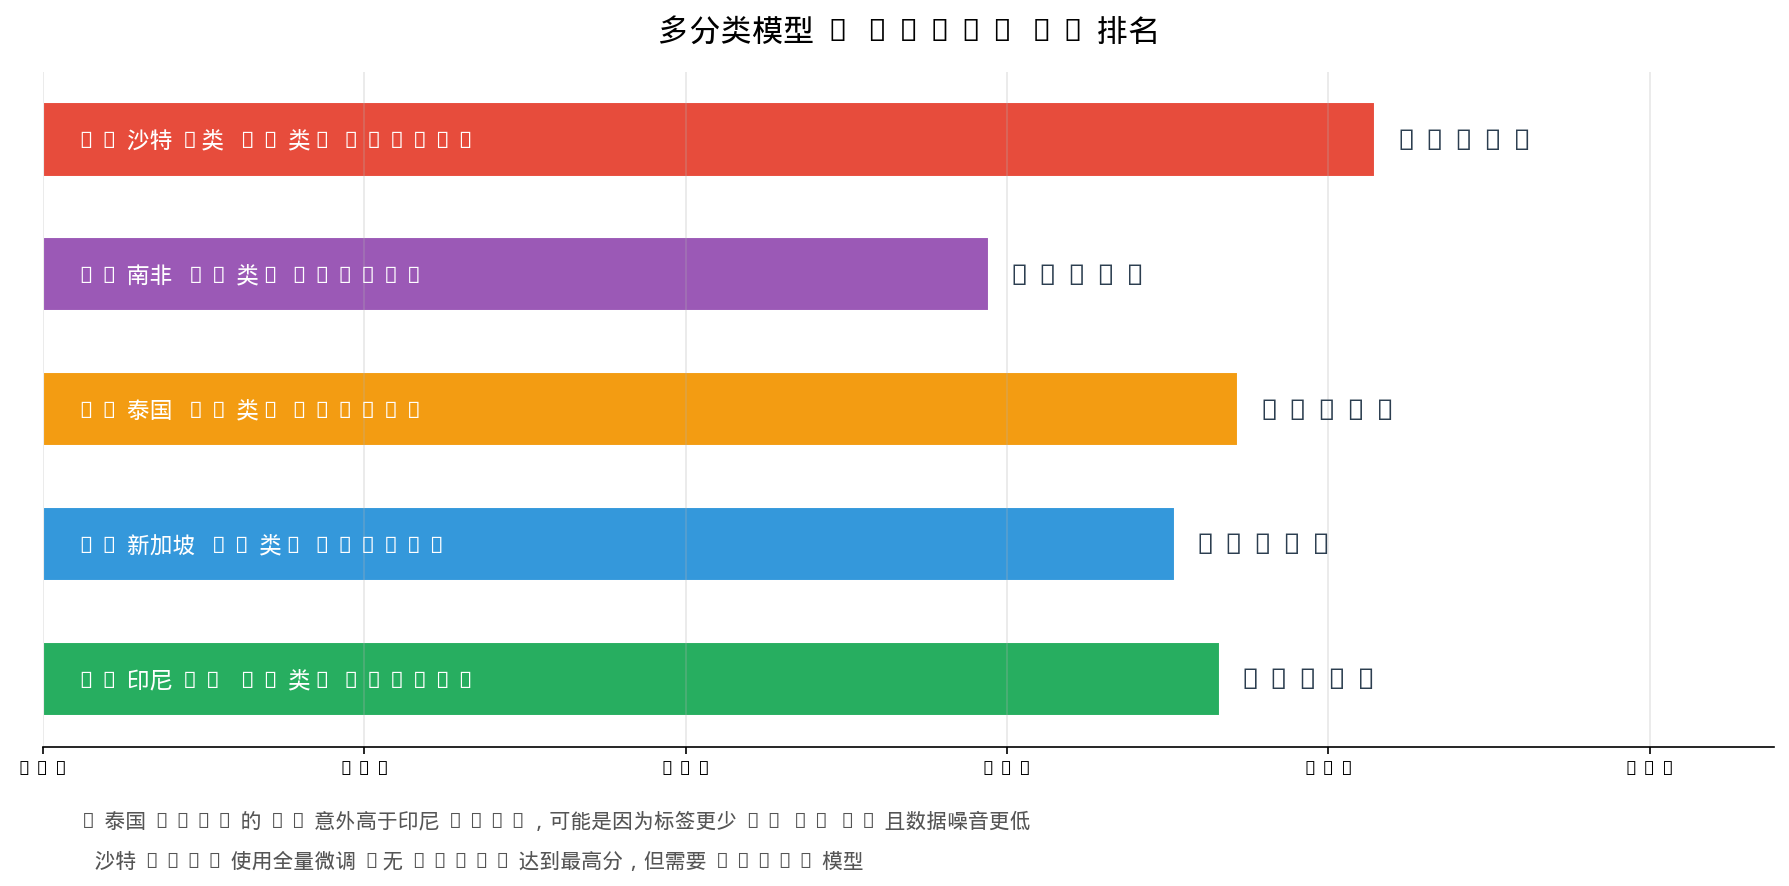
\includegraphics[width=0.85\textwidth]{charts/02_multiclass_ranking_cn.png}
\caption{多分类模型 Macro F1 排名}\label{fig:mc-rank}
\end{figure}

\begin{table}[h]\centering
\caption{多分类模型结果汇总}\label{tab:mc-results}
\begin{tabular}{@{}lrrrl@{}}
\toprule
\textbf{国家} & \textbf{标签数} & \textbf{训练量} & \textbf{Macro F1} & \textbf{训练方法} \\
\midrule
沙特 (SA) & 8 & $\sim$15K & \textbf{0.829} & 全量微调 \\
泰国 (TH) & 8 & 17,751 & \textbf{0.744} & LoRA LS + cal \\
印尼 (ID v6) & 9 & 45,753 & \textbf{0.732} & LoRA LS + cal \\
新加坡 (SG) & 9 & 25,543 & \textbf{0.704} & LoRA LS + cal \\
南非 (ZA) & 9 & 21,329 & \textbf{0.589} & LoRA LS + cal \\
\bottomrule
\end{tabular}
\end{table}

\subsection{各标签 F1 热力图}

\begin{figure}[h]\centering
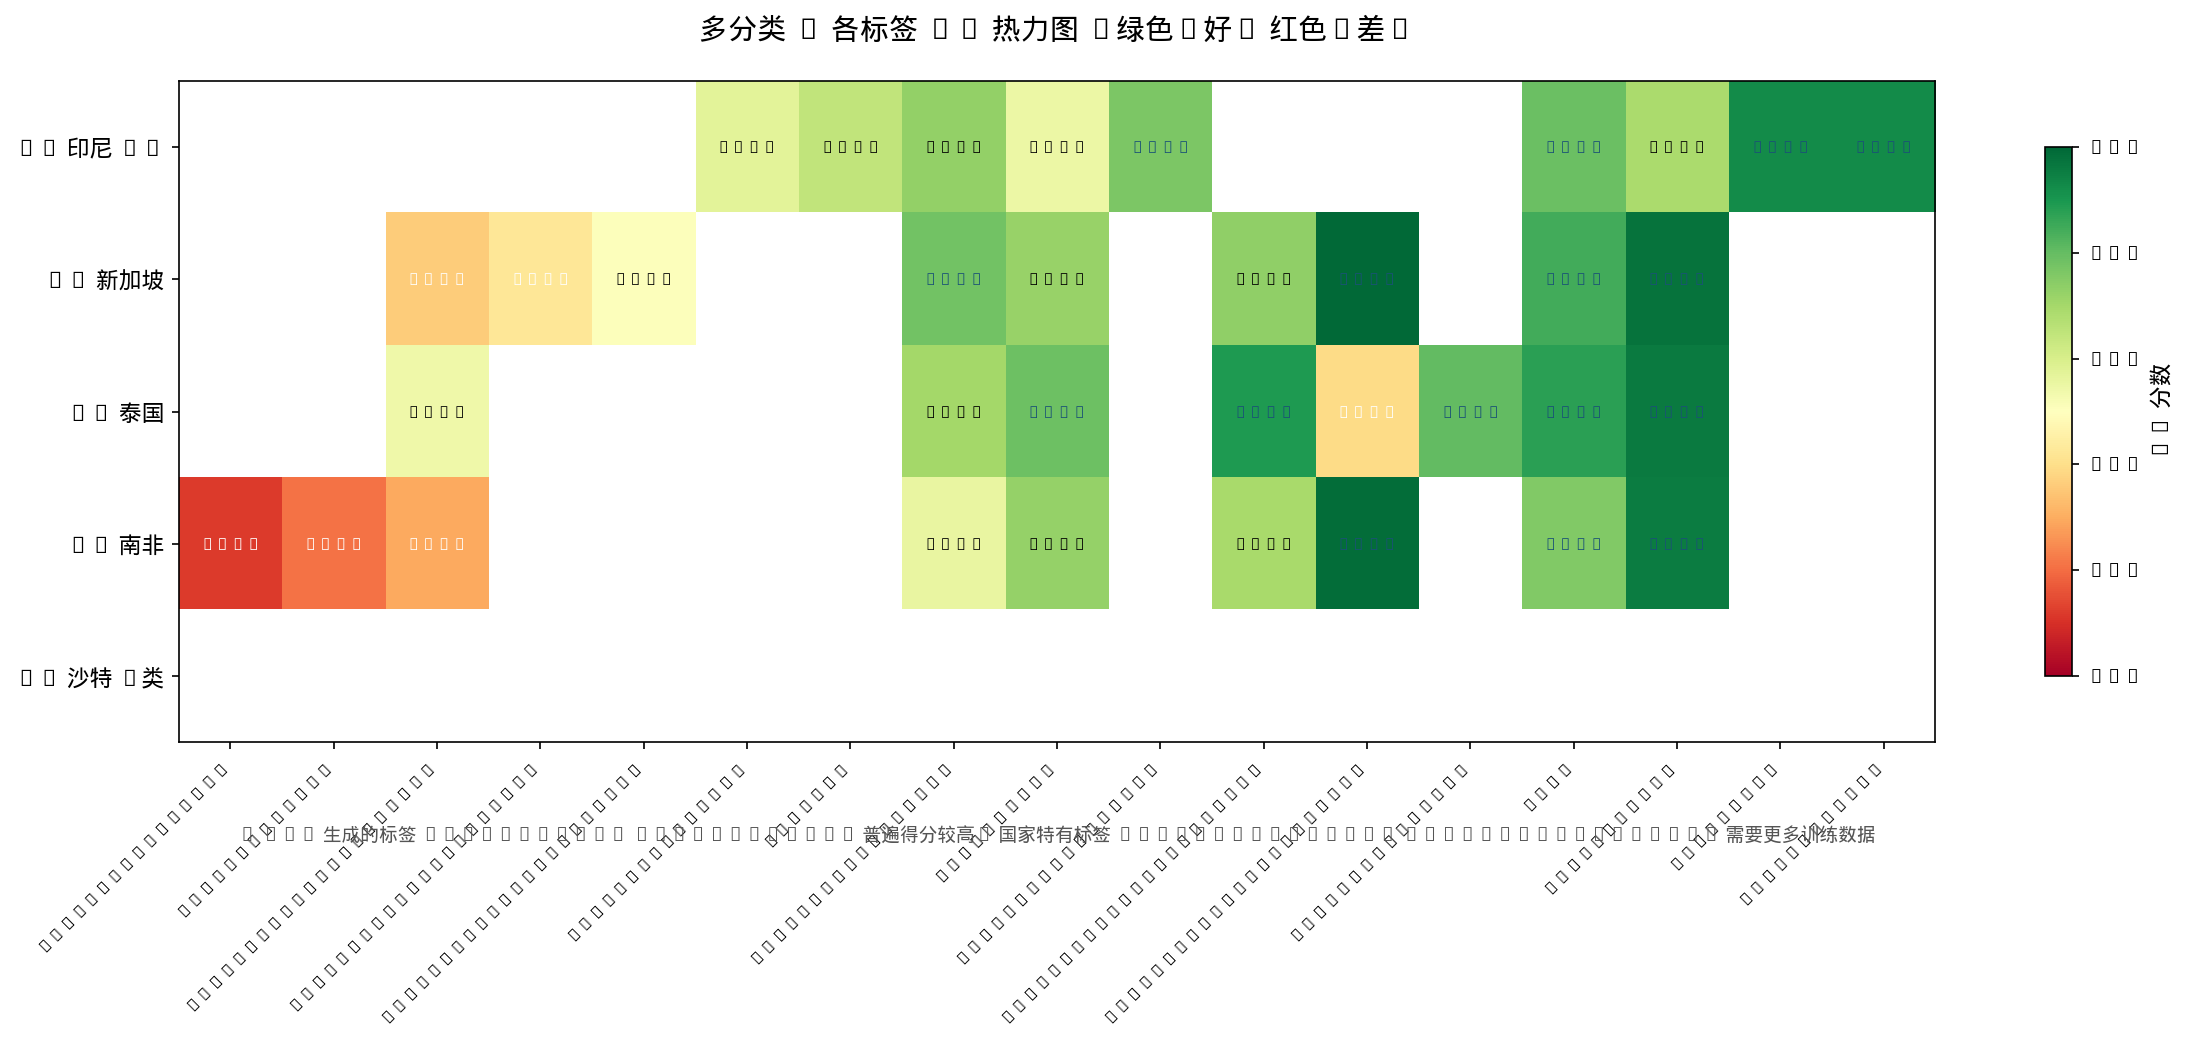
\includegraphics[width=\textwidth]{charts/03_multiclass_heatmap_cn.png}
\caption{各标签 × 各国 F1 热力图 (绿=好, 红=差)}\label{fig:heatmap}
\end{figure}

\subsection{印尼 (ID) — 最优模型详细结果}

印尼模型经过 6 个版本迭代，v6 达到最佳效果。

\begin{table}[h]\centering
\caption{ID v6 — 各类别完整结果}\label{tab:id-v6}
\begin{tabular}{@{}lrrrr@{}}
\toprule
\textbf{标签} & \textbf{Precision} & \textbf{Recall} & \textbf{F1} & \textbf{Support} \\
\midrule
Political & 1.000 & 0.855 & 0.922 & 145 \\
ID\_Blasphemy & 0.974 & 0.881 & 0.925 & 168 \\
safe & 0.787 & 0.793 & 0.790 & 2,088 \\
Sexually\_Explicit & 0.751 & 0.778 & 0.764 & 654 \\
Hate\_Speech & 0.810 & 0.599 & 0.689 & 866 \\
Dangerous\_Content & 0.714 & 0.747 & 0.730 & 982 \\
ID\_SARA & 0.674 & 0.624 & 0.648 & 822 \\
Harassment & 0.496 & 0.618 & 0.551 & 1,053 \\
other\_violation & 0.662 & 0.506 & 0.573 & 85 \\
\hline
\textbf{Overall} & — & — & \textbf{0.732} & 6,863 \\
\bottomrule
\end{tabular}
\end{table}

\subsection{泰国 (TH) — 详细结果}

\begin{table}[h]\centering
\caption{TH — 各类别完整结果}\label{tab:th}
\begin{tabular}{@{}lrrrr@{}}
\toprule
\textbf{标签} & \textbf{Precision} & \textbf{Recall} & \textbf{F1} \\
\midrule
Hate\_Speech & 0.936 & 0.982 & 0.959 \\
Sexually\_Explicit & 0.934 & 0.853 & 0.892 \\
safe & 0.863 & 0.888 & 0.875 \\
TH\_Lese\_Majeste & 0.792 & 0.814 & 0.803 \\
Harassment & 0.865 & 0.722 & 0.787 \\
Dangerous\_Content & 0.630 & 0.793 & 0.702 \\
Cybersecurity\_Malware & 0.754 & 0.422 & 0.541 \\
Politically\_Sensitive & 0.465 & 0.341 & 0.393 \\
\hline
\textbf{Overall} & — & — & \textbf{0.744} \\
\bottomrule
\end{tabular}
\end{table}

\subsection{新加坡 (SG) — 详细结果}

\begin{table}[h]\centering
\caption{SG — 各类别完整结果}\label{tab:sg}
\begin{tabular}{@{}lrrrr@{}}
\toprule
\textbf{标签} & \textbf{Precision} & \textbf{Recall} & \textbf{F1} \\
\midrule
Politically\_Sensitive & 0.990 & 0.997 & 0.993 \\
Hate\_Speech & 0.953 & 0.999 & 0.975 \\
safe & 0.865 & 0.828 & 0.846 \\
Dangerous\_Content & 0.772 & 0.791 & 0.781 \\
Sexually\_Explicit & 0.763 & 0.708 & 0.734 \\
Harassment & 0.759 & 0.683 & 0.719 \\
SG\_Racial\_Religious & 0.516 & 0.492 & 0.504 \\
SG\_Vulgarity\_Singlish & 0.363 & 0.513 & 0.425 \\
Cybersecurity\_Malware & 0.394 & 0.333 & 0.361 \\
\hline
\textbf{Overall} & — & — & \textbf{0.704} \\
\bottomrule
\end{tabular}
\end{table}

% ════════════════════════════════════════════════════
\section{模型演进: 印尼 ID v1 → v6}

\begin{figure}[h]\centering
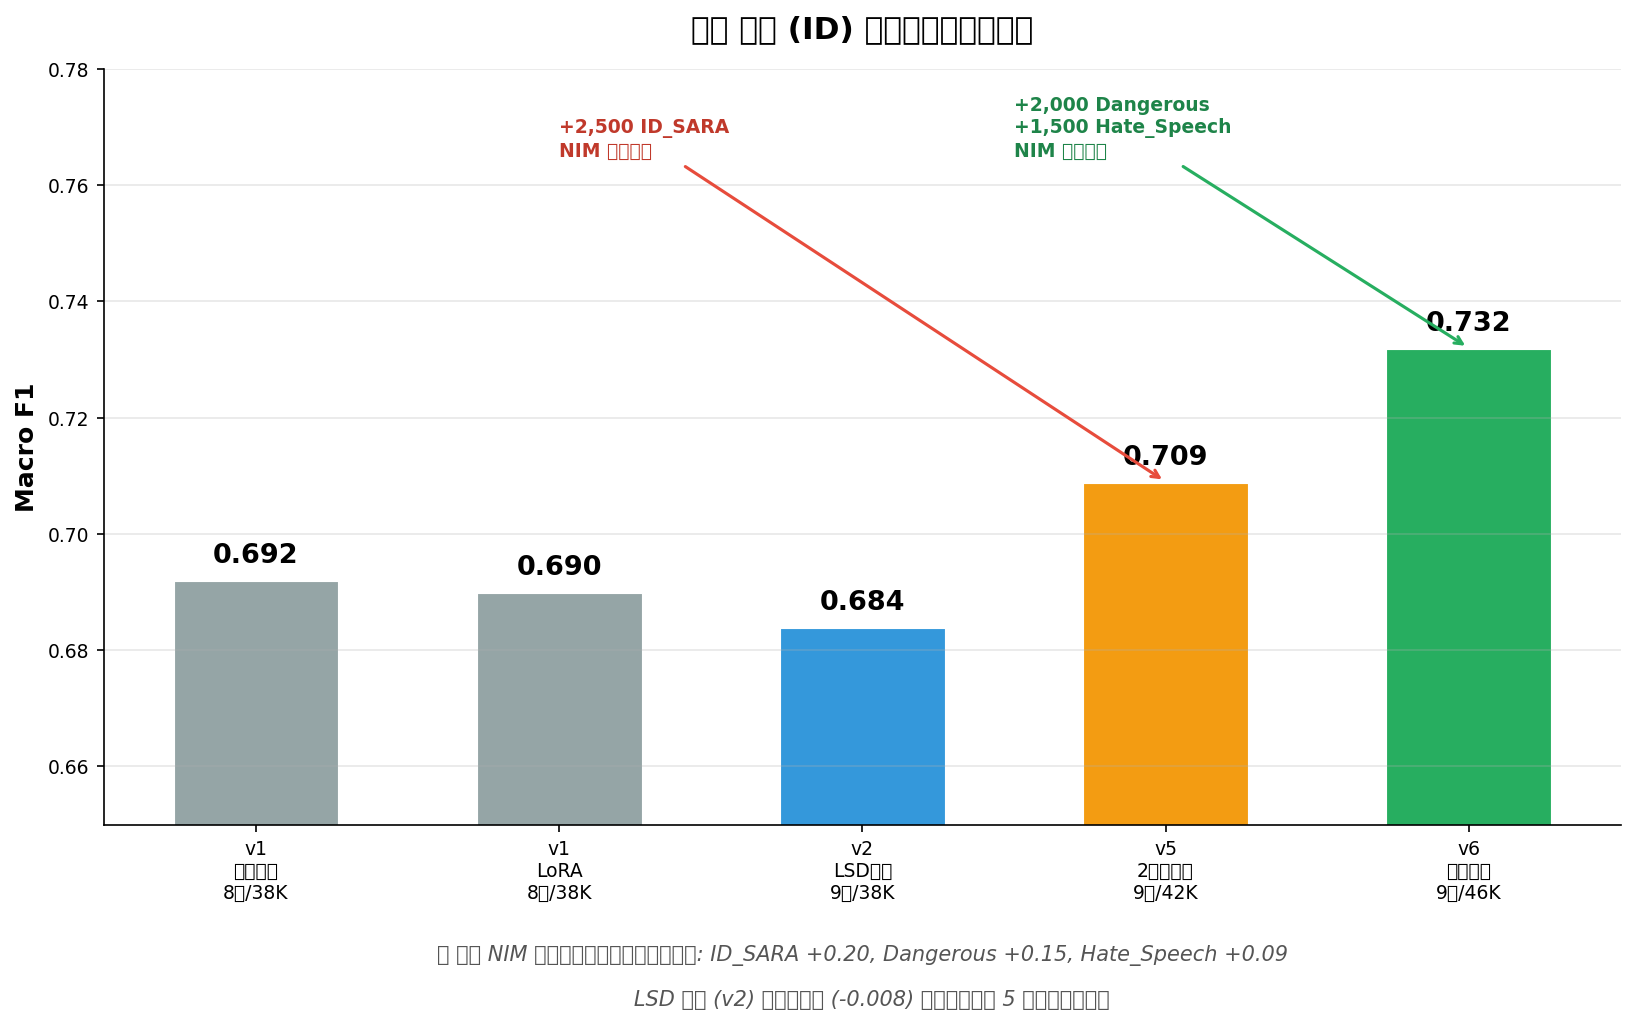
\includegraphics[width=0.9\textwidth]{charts/04_id_evolution_cn.png}
\caption{ID 模型 6 版本演进路线}\label{fig:id-evo}
\end{figure}

印尼模型经历了最完整的迭代优化:

\begin{enumerate}[itemsep=2pt]
\item \textbf{v1 (38K, 8-class)}: Full FT (0.692) 和 LoRA (0.690) 基线
\item \textbf{v2 (38K, 9-class)}: LSD 蒸馏尝试，F1 0.684，无明显提升
\item \textbf{v3}: 陪审团 relabeling，修正 ID\_SARA/Harassment 混淆
\item \textbf{v4}: NIM 生成 2,500 条 ID\_SARA 数据，ID\_SARA F1: 0.42 → 0.62
\item \textbf{v5 (42K)}: 2-seed LoRA LS ensemble + threshold calibration，F1 0.709
\item \textbf{v6 (46K)}: 补充 Dangerous\_Content (+2,000) + Hate\_Speech (+1,500)，
\textbf{F1 0.732}
\end{enumerate}

\textbf{核心经验}: NIM API 数据生成是提升弱势类别的最有效手段。

% ════════════════════════════════════════════════════
\section{综合仪表盘}

\begin{figure}[h]\centering
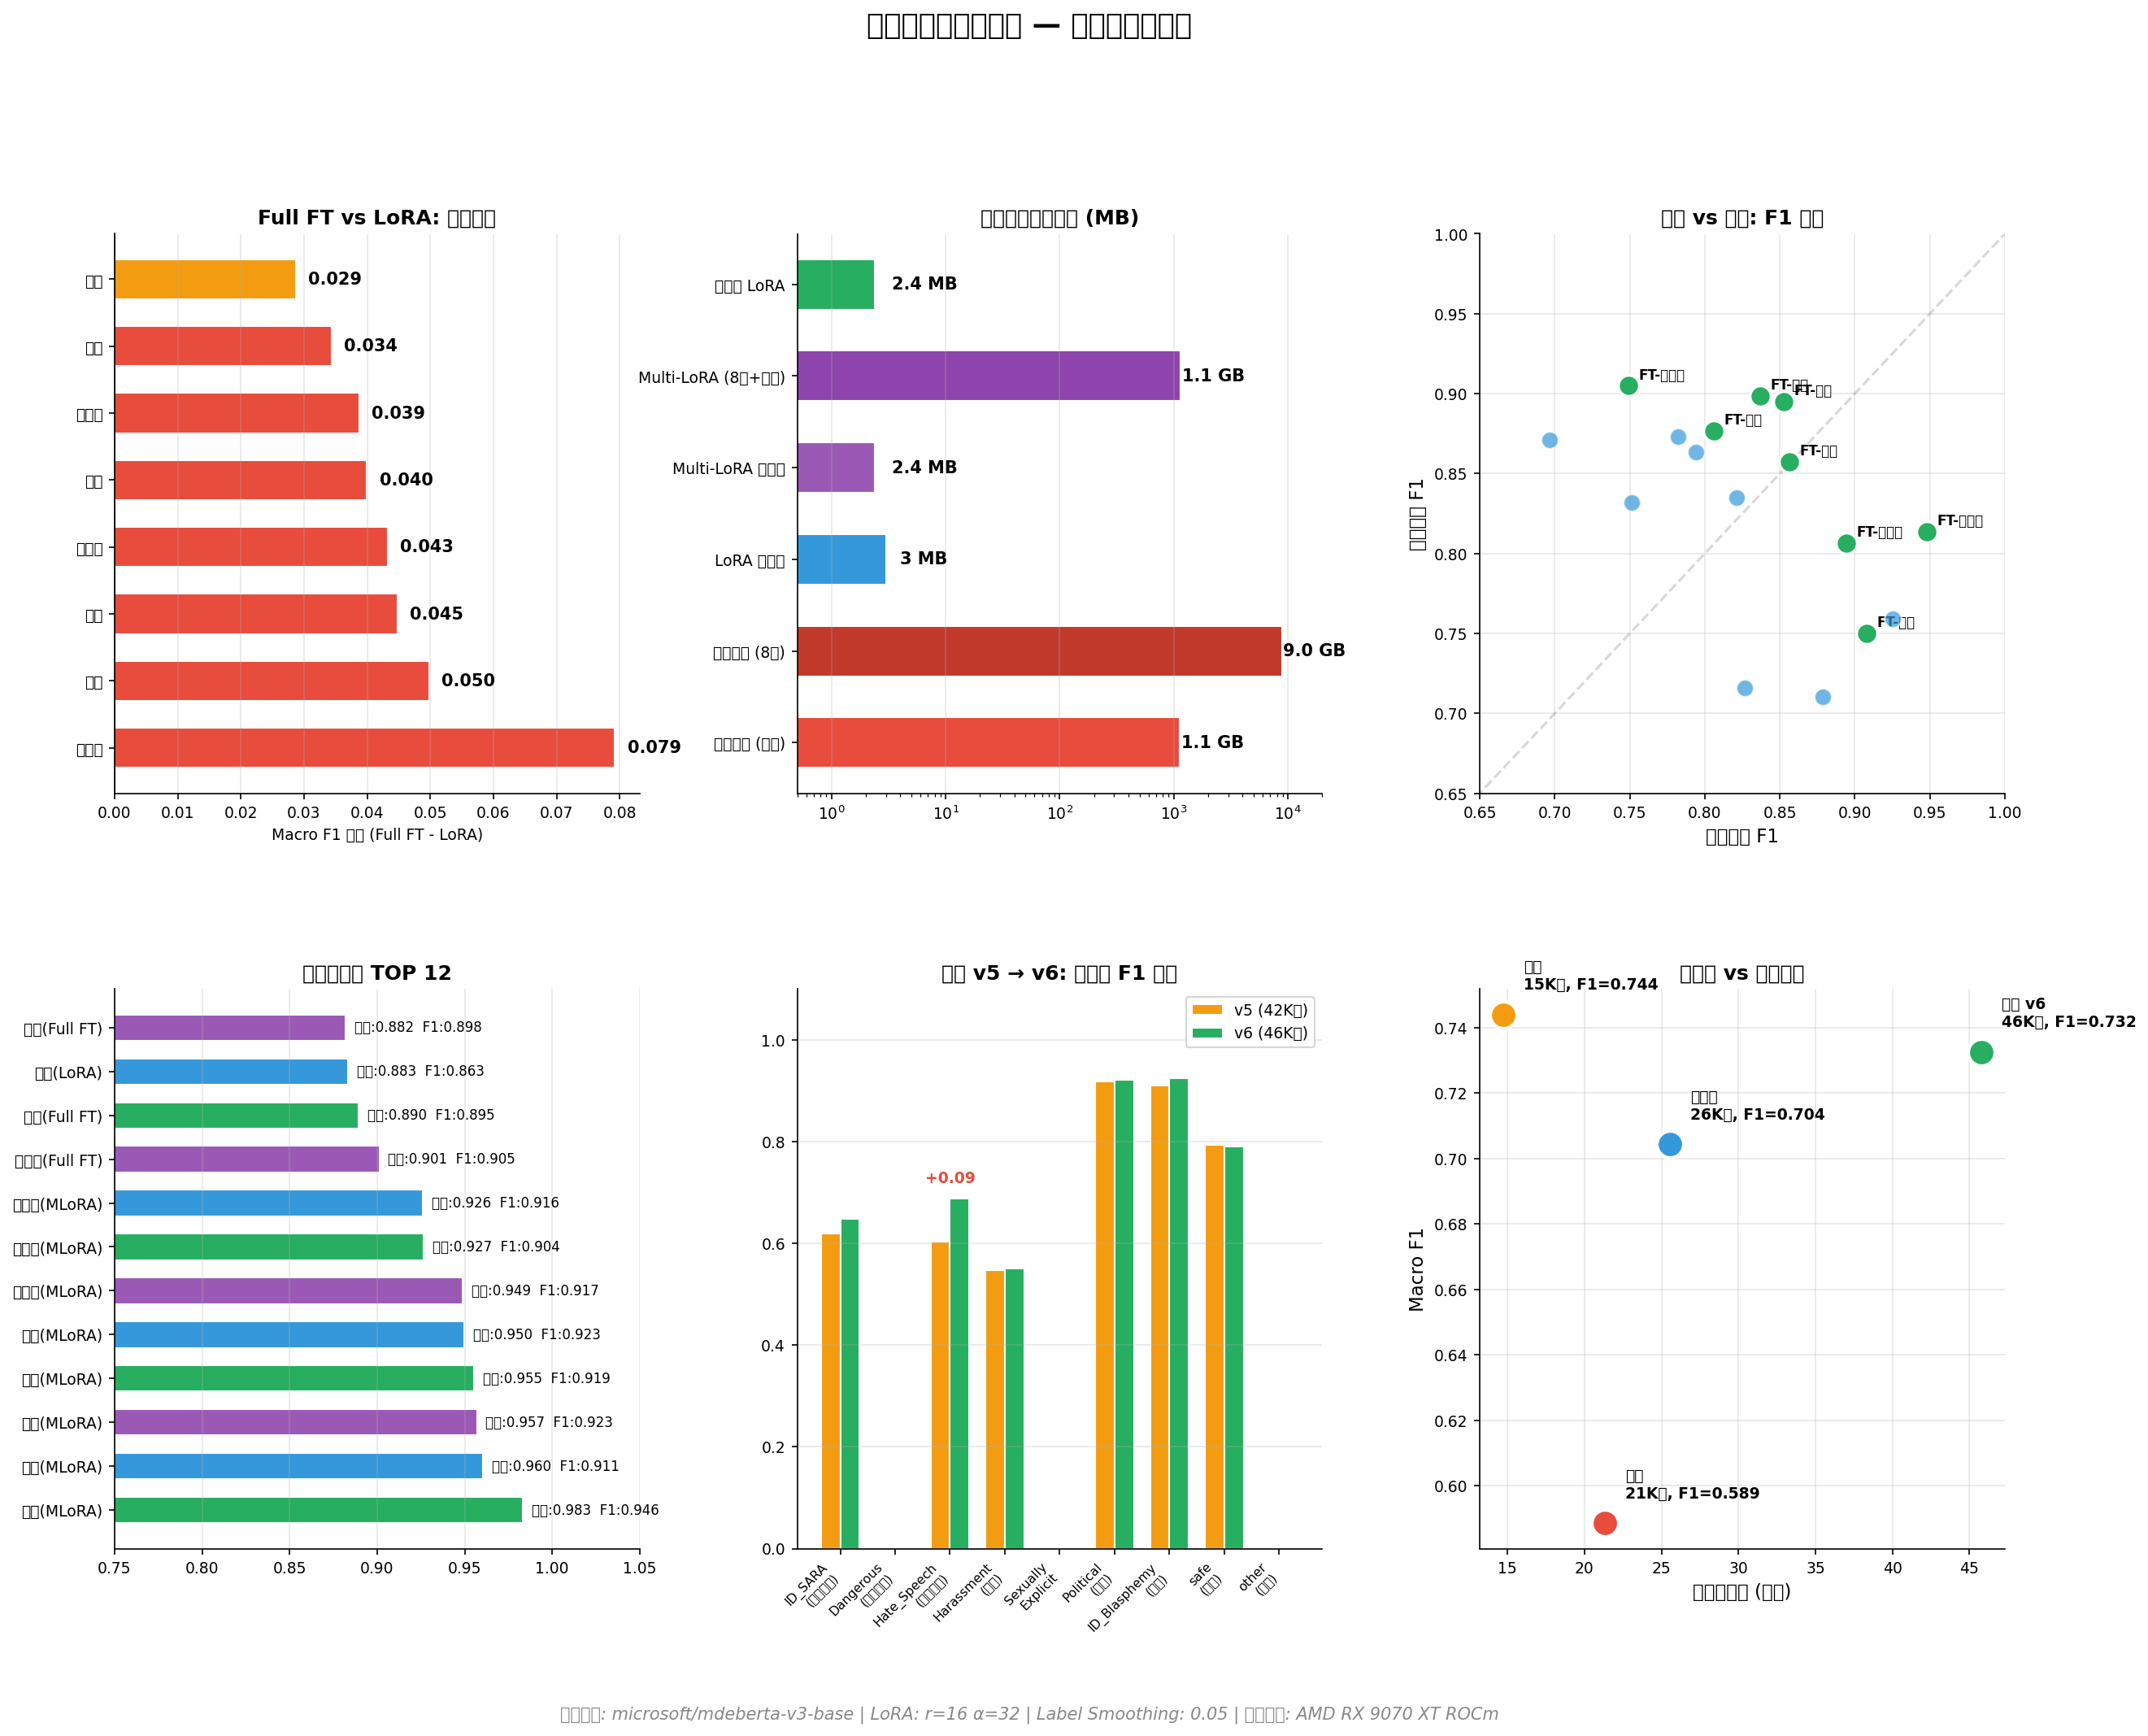
\includegraphics[width=\textwidth]{charts/05_dashboard_cn.png}
\caption{综合仪表盘 — 6 个维度全面对比}\label{fig:dashboard}
\end{figure}

\subsection{关键发现}

\begin{enumerate}[itemsep=3pt]
\item \textbf{全量微调在所有二分类任务中都是最优方法}，
平均 Macro F1 达到 0.853，比 LoRA 高 0.044，比 Adapter 高 0.084。
\item \textbf{Multi-LoRA 违规召回率最高}但安全内容召回率低，
倾向于将所有内容判为违规，容易误报。
\item \textbf{多分类中泰国 (TH) 表现意外好于印尼 (ID)}，
可能因为标签更少 (8 vs 9) 且数据标注质量更高。
\item \textbf{NIM 数据生成是最有效的模型改进手段}，
ID\_SARA (+0.23)、Dangerous (+0.15)、Hate\_Speech (+0.09)。
\item \textbf{LSD 蒸馏不推荐}，训练慢 5 倍但提升不足 0.01。
\item \textbf{Label Smoothing (0.05) 稳定优于普通 CrossEntropy}。
\item \textbf{Threshold calibration 提供 +0.01-0.02 的免费提升}。
\item \textbf{模型存储效率}: LoRA 适配器仅 2.4MB，
比全量微调 (1.1GB) 小 460 倍，适合多国部署。
\end{enumerate}

% ════════════════════════════════════════════════════
\section{模型部署}

\subsection{HuggingFace Hub}

所有模型已上传至 HuggingFace Hub:
\url{https://huggingface.co/jianqiang0213}

\begin{table}[h]\centering
\caption{HF 模型命名规则}\label{tab:hf-names}
\begin{tabular}{@{}ll@{}}
\toprule
\textbf{类型} & \textbf{Repo ID} \\
\midrule
二分类 Full FT & \texttt{mdeberta-v3-\{COUNTRY\}-binary-fullft} \\
二分类 LoRA & \texttt{mdeberta-v3-\{COUNTRY\}-binary-lora} \\
二分类 Multi-LoRA & \texttt{mdeberta-v3-\{COUNTRY\}-binary-multilora} \\
多分类 LoRA & \texttt{mdeberta-v3-\{COUNTRY\}-multiclass-lora} \\
\bottomrule
\end{tabular}
\end{table}

\subsection{使用方法}

\subsubsection{二分类 Full FT}

\begin{verbatim}
from transformers import AutoModelForSequenceClassification, AutoTokenizer
model = AutoModelForSequenceClassification.from_pretrained(
    "jianqiang0213/mdeberta-v3-SG-binary-fullft"
)
tokenizer = AutoTokenizer.from_pretrained(
    "jianqiang0213/mdeberta-v3-SG-binary-fullft"
)
\end{verbatim}

\subsubsection{二分类 LoRA (PEFT)}

\begin{verbatim}
from peft import PeftModel
base = AutoModelForSequenceClassification.from_pretrained(
    "microsoft/mdeberta-v3-base", num_labels=2)
model = PeftModel.from_pretrained(
    base, "jianqiang0213/mdeberta-v3-SG-binary-lora")
\end{verbatim}

\subsubsection{多分类 LoRA}

\begin{verbatim}
base = AutoModelForSequenceClassification.from_pretrained(
    "microsoft/mdeberta-v3-base", num_labels=9)
model = PeftModel.from_pretrained(
    base, "jianqiang0213/mdeberta-v3-ID-v6-multiclass-lora")
\end{verbatim}

% ════════════════════════════════════════════════════
\section{未来工作}

\begin{enumerate}[itemsep=2pt]
\item \textbf{补充弱势类别数据}: ZA\_Xenophobia (F1=0.21) 和 ZA\_Severe\_Racism
(F1=0.12) 急需 NIM 生成补充 (类似 ID\_SARA 策略)
\item \textbf{扩展覆盖国家}: 巴西 (BR)、墨西哥 (MX)、土耳其 (TR) 的多分类模型尚未训练
\item \textbf{Multi-LoRA 多分类}: 将二分类 Multi-LoRA 架构升级为多分类，
实现一个基座服务 8 国 9 类违规检测
\item \textbf{模型集成}: 增加 seed 数量到 3 个以上，使用 soft voting 提升稳定性
\item \textbf{实际部署测试}: 在真实流量上进行 A/B 测试，验证离线指标与实际效果的一致性
\item \textbf{泰国和新加坡的 NIM 生成标签过拟合问题}: Political/Hate\_Speech 的
接近完美的 F1 表明这些标签存在 NIM 生成数据的特征泄露，需要用真实标注数据验证
\end{enumerate}

% ════════════════════════════════════════════════════
\section*{附录: 模型文件索引}

\begin{verbatim}
Training/model_reports/
├── binary/           # 二分类报告 (32 模型 × 4 方法)
│   ├── fullft/       #   Full FT (8 国)
│   ├── lora/         #   LoRA PEFT (8 国)
│   ├── multilora/    #   Multi-LoRA (8 国)
│   ├── adapter/      #   Adapter (8 国)
│   ├── shared/       #   架构对比
│   └── usage_guide.py
├── multiclass/       # 多分类报告 (5 国)
│   ├── id/           #   ID 6 版本演进
│   ├── sa/           #   SA 8-class FT
│   ├── sg/           #   SG 9-class
│   ├── th/           #   TH 8-class
│   └── za/           #   ZA 9-class
└── charts/           # 对比图表 (6 张)
\end{verbatim}

\vspace{1cm}
\begin{center}
\large\textbf{—— 完 ——}
\end{center}

\end{document}
